\icode{E-MI-MU-L3-261111-001}
如图所示，\(a\)、\(b\)是由同种材料构成的两物体，质量分别为\(m_1\)、\(m_2\)	，由轻质弹簧相连，放置在倾角为\(\theta\)的光滑的斜面上。当给物体\(a\)施加一沿斜面向上的恒力\(F\)时，两物体一起斜向上做加速度为\(a\)的匀加速直线运	动，此时弹簧的伸长量为\(x\)，则\paren[]

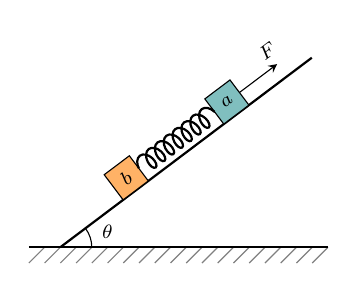
\begin{tikzpicture}[>=stealth,font=\scriptsize]
	\begin{scope}[rotate=37]
		\draw[thick] (0,0)--(4,0);
		\draw[fill=orange!60] (1,0) rectangle(1.4,.4)node[midway,rotate=37]{\(b\)};
        \draw[fill=teal!50] (2.6,0) rectangle(3,.4)node[midway,rotate=37]{\(a\)};
		\draw[thick,decoration={aspect=.6,segment length=4,amplitude=1.2mm,coil},decorate] (1.4,.2)--(2.6,.2);
		\draw[->] (3,.2)--(3.6,.2)node[above,rotate=37]{\(F\)};
	\end{scope}
	\foreach \x in {-.4,-.2,...,3.2}
		\draw[gray] (\x,-.2)--++(.2,.2);
	\draw[thick] (-.4,0)--(3.4,0);
	\draw (.4,0) arc(0:37:.4);
	\node at(.6,.2){\(\theta\)};
\end{tikzpicture}
\begin{choices}
	\item 弹簧的劲度系数为\(k = \dfrac{F - m_2g\sin\theta}{x}\)
	\item 弹簧的劲度系数为\(k = \dfrac{m_1F}{(m_1 + m_2)x}\)
	\item 在运动过程中，若突然撤去拉力\(F\)，则撤去\(F\)的瞬间\(a\)物体的加速度大小为\(\dfrac{F}{m_1} - a\)
		\item 若斜面粗糙，在同样恒力\(F\)作用下，两物体仍能斜向上匀加速运动，弹簧的伸长量将大于\(x\)
\end{choices}
\begin{answer}
    AD\qquad 提示：
\end{answer}